\documentclass[a4paper,11pt,twocolumn]{article}
\usepackage{fancyhdr}
\usepackage{enumerate}
\usepackage{times}
\usepackage{mathptmx}
\usepackage{amsmath}
\usepackage{amsfonts}
\usepackage{amssymb}
\usepackage{tikz}
\usepackage{clrscode3e}
\usepackage[top=2cm, bottom=2cm, left=2cm, right=2cm]{geometry}

\setlength{\columnsep}{7mm}

\newcommand{\homeworkno}{3.1}
\pagestyle{fancy}
\lhead{Problem Solving: Homework \homeworkno}
\chead{}
\rhead{Chen Shaoyuan (161240004)}
\lfoot{}
\cfoot{\thepage}
\rfoot{}

\newcommand{\NIL}{\const{nil}}
\newcommand{\FALSE}{\const{false}}
\newcommand{\TRUE}{\const{true}}

\allowdisplaybreaks[4]
\renewcommand{\labelenumi}{\textbf{\emph{\alph{enumi}}.}}
\begin{document}
  \title{Problem Solving: Homework \homeworkno}
  \author{Name: Chen Shaoyuan \and Student ID: 161240004}
  \maketitle

  \section{[TC] Problem 24.1-2}
  We claim that, after $k$ passes of relaxation, $\attrib{v}{d} < \infty$ holds if $d(s, v) \leq k$. This can be proved by mathematical induction: for the base step, only the source $s$ satisfies $s.d = 0 < \infty$, and the conclusion is true; for the induction step, assume that before the $i$-th pass of relaxation, for every vertex $v$ such that $d(s, v) < i$,  $\attrib{v}{d} < \infty$. When performing relaxation, an estimate $v.d$ is changed from infinity to a finite number, if and only if there exists a directed edge $(u, v)$, such that $u.d < \infty$ and $v.d = \infty$. Therefore, for all vertices $v$ such that $d(s, v) = i$, $\attrib{v}{d} < \infty$. By mathematical induction, we prove the correctness of the claim. \par
  Note that, if there exists a path from $s$ to $v$, then $d(s, v) < |V|$ always holds, and Bellman-Ford algorithm performs $|V|-1$ passes of relaxation in total. If for all vertices $v$, there exists a path from $s$ to $v$, then the algorithms must terminate with $\attrib{v}{d} < \infty$. Otherwise, if there exists a vertex $v$, such that $v$ is unreachable from $s$, then it remains $\attrib{v}{d} = \infty$ when algorithm terminates. This is because, $\attrib{v}{d}$ is always an upper bound of $\delta(s, v)$ which is infinity, so every relaxation attempting to tighten $\attrib{v}{d}$ will not succeed.

  \section{[TC] Problem 24.1-3}
  We use a flag to record whether a relaxation succeeds in a pass of relaxation. When no relaxation succeeds in a pass, we terminate the algorithm. The total number of passes executed is $m+1$.

  \section{[TC] Problem 24.1-4}
  \begin{codebox}
  \Procname{$\proc{Bellman-Ford-Modified}(G,w,s)$}
  \li $\proc{Initialize-Single-Source}(G,S)$
  \li \For $i \gets 1$ to $|\attrib{G}{V}|-1$
  \li \Do  \For each edge $(u, v) \in \attrib{G}{E}$
  \li      \Do  $\proc{Relax}(u, v, w)$
           \End
      \End
  \li Let $Q$ be a new queue of vertices
  \li \For each vertex $v \in \attrib{G}{V}$
  \li \Do  $\attrib{v}{flag} = \FALSE$
      \End
  \li \For each edge $(u, v) \in \attrib{G}{E}$
  \li \Do  \If $\attrib{v}{d} > \attrib{u}{d} + w(u, v)$
  \li      \Do $\attrib{Q}{enqueue}(v)$
  \li          $\attrib{v}{flag} \gets \TRUE$
           \End
      \End
  \li \While $Q$ is not empty
  \li \Do    $u \gets \attrib{Q}{dequeue}()$
  \li        \For each $v \in \attrib{u}{adj}$
  \li        \Do  $\attrib{v}{d} = -\infty$
  \li             \If $\attrib{v}{flag} \isequal \FALSE$
  \li             \Do $\attrib{Q}{enqueue}(v)$
  \li                 $\attrib{v}{flag} \gets \TRUE$
                  \End
             \End
      \End
  \end{codebox}

  \section{[TC] Problem 24.2-2}
  After changing, only the last vertex in topological order is not taken. However, the last vertex does not have successor, therefore, the procedure remains correct.

  \section{[TC] Problem 24.3-2}
  \small
  \begin{center}
  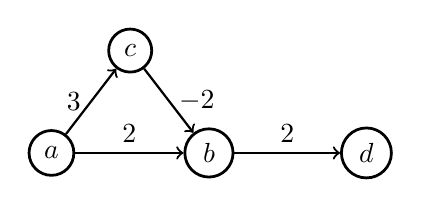
\begin{tikzpicture}[line width = 1pt,
                        solid/.style = {circle, draw, fill = black, minimum size = 0.1cm},
                        empty/.style = {circle, draw, fill = white, minimum size = 0.1cm}]
    \node [empty] (a) at (0, 0){$a$};
    \node [empty] (b) at (2, 0){$b$};
    \node [empty] (c) at (1, 1.3){$c$};
    \node [empty] (d) at (4, 0){$d$};
    \draw [thick,->] (a)--(b) node[midway,above] {$2$};
    \draw [thick,->] (a)--(c) node[midway,left] {$3$};
    \draw [thick,->] (c)--(b) node[midway,right] {$-2$};
    \draw [thick,->] (b)--(d) node[midway,above] {$2$};
  \end{tikzpicture} \par
  \end{center}
  \normalsize
  Consider the graph shown above, if we take $a$ as the source and run Dijkstra's algorithm, the procedure adds $a$, $b$, $c$, $d$ to set $S$ and relaxes edges $(a, b), (a, c)$; $(b, d)$; $(c, b)$. It finally terminates with $\attrib{a}{d} = 0$, $\attrib{b}{d} = 1$, $\attrib{c}{d} = 3$, $\attrib{d}{d} = 4$. Note that for vertex $d$, we have path $\langle a, c, b, d \rangle$ whose length is 3, which means Dijkstra's algorithm gives wrong answer. \par
  In the \textbf{maintenance} part of the proof, formula (24.2) holds because all edges are non-negative. If negative edges are allowed, the formula no longer holds and the $\attrib{u}{d} = \delta(s, u)$ might not hold for vertex $u$ added to set $S$.

  \section{[TC] Problem 24.3-4}
  \begin{codebox}
  \Procname{$\proc{Dijkstra-Checker}(G, w, s)$}
  \li \If $\attrib{s}{d} \neq 0$ or $\attrib{\pi} \neq \NIL$
  \li \Do \Return \FALSE
      \End
  \li \For each vertex $v \in \attrib{G}{V}$
  \li \Do  $\attrib{v}{d'} \gets \infty$
      \End
  \li $\attrib{s}{d'} \gets 0$
  \li \For each edge $(u, v) \in \attrib{G}{E}$
  \li \Do  $\attrib{v}{d'} \gets \min(\attrib{v}{d}, \attrib{u}{d} + w(u, v))$
      \End
  \li \For each vertex $v \in \attrib{G}{V}$
  \li \Do \If $v \neq s$
  \li     \Do \If $\attrib{v}{d} \neq \attrib{v}{d'}$
  \li         \Do \Return \FALSE
              \End
  \li     \If $\attrib{v}{\pi} \neq \NIL$
  \li         \Do \If $\attrib{v}{d} \neq \attribb{v}{\pi}{d} + w(\attrib{v}{\pi}, v)$
  \li             \Do \Return \FALSE
                  \End
  \li         \ElseIf $\attrib{v}{d} \neq \infty$
  \li         \Do \Return \FALSE
              \End
          \End
      \End
  \li \Return \TRUE
  \end{codebox}

  \section{[TC] Problem 24.3-7}
  $G'$ has $|V| + \sum_{e \in E} [w(e)-1]$ vertices. \par
  In breadth first-first search, a vertices $v$ with less $d_{G'}(s, v)$ are colored black before one with larger $d_{G'}(s, v)$. For vertices $v \in V$, $d_{G'}(s, v) = \delta_G(s, v)$. In Dijkstra's algorithm, a vertex $v$ with smallest $\attrib{v}{d}$ is extracted from priority queue, and we've proved that $\attrib{v}{d} = \delta_{G}(s, v)$. So, both breadth-first search and Dijkstra's algorithm repeat coloring or extracting vertex $v \in V$ with least $\delta_{G}(s, v)$, and since $\delta_{G}(s, v)$ are distinct, the two orders are same.

  \section{[TC] Problem 24.5-2}
  \small
  \begin{center}
  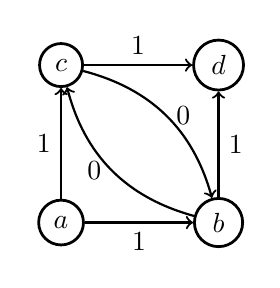
\begin{tikzpicture}[line width = 1pt,
                        solid/.style = {circle, draw, fill = black, minimum size = 0.1cm},
                        empty/.style = {circle, draw, fill = white, minimum size = 0.1cm}]
    \node [empty] (a) at (0, 0){$a$};
    \node [empty] (b) at (2, 0){$b$};
    \node [empty] (c) at (0, 2){$c$};
    \node [empty] (d) at (2, 2){$d$};
    \draw [thick,->] (a)--(b) node[midway,below] {$1$};
    \draw [thick,->] (a)--(c) node[midway,left] {$1$};
    \draw [thick,->] (b)--(d) node[midway,right] {$1$};
    \draw [thick,->] (c)--(d) node[midway,above] {$1$};
    \draw [thick,->] (b) edge [bend left=30] node[midway,left] {$0$} (c);
    \draw [thick,->] (c) edge [bend left=30] node[midway,right] {$0$} (b);
  \end{tikzpicture} \par
  \end{center}
  \normalsize
  Consider the graph above, take $a$ as the source, then trees consisting of edges $(a, b), (b, d), (b, c)$ and $(a, c), (c, d), (c, b)$ are both shortest-paths trees rooted at $a$, and for every edge $e \in E$, exactly one of the two trees contains $e$.

  \section{[TC] Problem 24.5-5}
  \small
  \begin{center}
  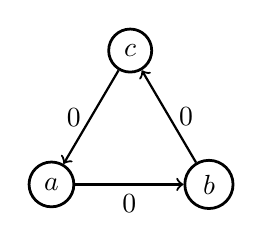
\begin{tikzpicture}[line width = 1pt,
                        solid/.style = {circle, draw, fill = black, minimum size = 0.1cm},
                        empty/.style = {circle, draw, fill = white, minimum size = 0.1cm}]
    \node [empty] (a) at (0, 0){$a$};
    \node [empty] (b) at (2, 0){$b$};
    \node [empty] (c) at (1, 1.7){$c$};
    \draw [thick,->] (a)--(b) node[midway,below] {$0$};
    \draw [thick,->] (b)--(c) node[midway,right] {$0$};
    \draw [thick,->] (c)--(a) node[midway,left] {$0$};
  \end{tikzpicture} \par
  \end{center}
  \normalsize

  Consider the graph above, let $a$ be the source vertex. If we take $\attrib{a}{\pi} = c$, $\attrib{b}{\pi} = a$, $\attrib{c}{\pi} = b$, then they form a cycle.

  \section{[TC] Problem 24-2}
  \begin{enumerate}
  \item If box $A$ with dimensions $(x_1, x_2, \cdots, x_d)$ nests in box $B$ with dimensions $(y_1, y_2, \cdots, y_d)$, box $B$ nests in box $C$ with dimensions $(z_1, z_2, \cdots, z_d)$, then there exist permutations $\pi_1, \pi_2$ on $\{1, 2, \cdots, d\}$, such that
  $$ x_{\pi_1(1)} < y_1, x_{\pi_1(2)} < y_2, \cdots, x_{\pi_1(d)} < y_d $$
  $$ y_{\pi_2(1)} < z_1, y_{\pi_2(2)} < z_2, \cdots, y_{\pi_2(d)} < z_d $$
  therefore
  $$ x_{\pi_1(\pi_2(1))} < z_1, x_{\pi_1(\pi_2(2))} < z_2, \cdots, x_{\pi_1(\pi_2(d))} < z_d $$
  note that $\pi_1 \circ \pi_2$ is still a permutation, so box $A$ nests in box $C$, i.e. the nesting relation is transitive.
  \item Given boxes $A$ with dimensions $(x_1, x_2, \cdots, x_d)$ and $B$ with dimensions $(y_1, y_2, \cdots, y_d)$. Sort $(x_1, x_2, \cdots, x_d)$ and $(y_1, y_2, \cdots, y_d)$ in increasing order respectively, then check whether there exists $i (1 \leq i \leq d)$, such that $x_i \geq y_i$. If exists, then $A$ does not nest in $B$; otherwise, $A$ nests in $B$. \par
  Assume that array $(y_1, y_2, \cdots, y_n)$ is sorted in increasing order. For array $(x_1, x_2, \cdots, x_n)$ which is not sorted in increasing order, there must exist an inversion pair $(x_i, x_j)$ ($x_i>x_j, i<j$). If $x_i < y_i$ and $x_j < y_j$, since $x_i > x_j$, $y_i < y_j$, we have $x_j < y_i$ and $x_i < y_j$, so after exchanging $x_i$ with $x_j$, the condition still holds. Since any finite permutation can be generated by swapping, greedy algorithm applies here and the method mentioned before is correct.
  \item The pseudocode is shown in the next page.
  \begin{codebox}
  \Procname{$\proc{Longest-Nested-Boxes}(B, n)$}
  \li $maxd \gets 0$
  \li \For $i \gets 1$ to $n$
  \li \Do  sort dimensions of $B_i$ in increasing order
  \li      $\attrib{B_i}{d} \gets 0$
  \li      $\attrib{B_i}{\pi} \gets \NIL$
      \End
  \li \For $i \gets 1$ to $n$
  \li \Do  \For $j \gets 1$ to $n$
  \li      \Do  \If $B_i$ is nested in $B_j$
  \li           \Do $\attribb{B_j}{adj}{insert}(i)$
                \End
           \End
      \End
  \li \For every $B_i$ in $B$ in topological order
  \li \Do  \For every $j$ in $\attrib{B_i}{adj}$
  \li      \If  $\attrib{B_j}{d} < \attrib{B_i}{d} + 1$
  \li      \Do  $\attrib{B_j}{d} \gets \attrib{B_i}{d} + 1$
  \li           $\attrib{B_j}{\pi} \gets B_i$
  \li           \If $\attrib{B_j}{d} > maxd$
  \li           \Do $maxd \gets \attrib{B_j}{d}$
  \li               $r \gets B_j$
                \End
           \End
      \End
  \li \While $r \neq \NIL$
  \li \Do print $r$
  \li     $r \gets \attrib{r}{\pi}$
      \End
  \end{codebox}

  This algorithm first builds a graph $G$, in which edge $(u, v)$ means that $v$ is nested in $u$. Then it calculates the longest nested boxes ending in $v$ in topological order. Since we presorted the dimensions of all the boxes in $O(nd \log d)$ time, determining whether one box nests in another takes only $O(d)$ time, and thus building the graph takes $O(n^2d)$ in all. Calculating the longest nested boxes takes $O(|V|+|E|) = O(n^2)$ time. Therefore, the total running time is $O(nd \log d + n^2d)$.
  \end{enumerate}

  \section{[TC] Problem 24-3}
  \begin{enumerate}
  \item First, build a graph $G=(V, E)$, where $V = \{c_1, c_2, \cdots, c_n\}$, $E = \{(i, j)| i, j \in V\}$, and $w(i, j) = \ln R[i,j]$. Then we run Bellman-Ford algorithm on $G$ to determine whether negative-weight cycle. Such sequence exists if and only if $G$ contains negative-weight cycle. The running time is $O(|V||E|) = O(n^3)$.
  \item In the following procedure, assume that Bellman-Ford algorithm has been performed on $G$.
  \begin{codebox}
  \Procname{$\proc{Find-Sequence}(G)$}
  \li \For every vertex $v \in \attrib{G}{V}$
  \li \Do  $\attrib{v}{flag} \gets 0$
      \End
  \li $cnt \gets 0$
  \li \For every vertex $v \in \attrib{G}{V}$
  \li \Do $u \gets v$
  \li     $cnt \gets cnt + 1$
  \li     \While $u \neq \NIL$ and $\attrib{u}{cnt} \isequal 0$
  \li     \Do $\attrib{u}{flag} \gets cnt$
  \li         $u \gets \attrib{u}{\pi}$
  \li         \If $u \neq \NIL$ and $\attrib{u}{flag} \isequal cnt$
  \li         \Do print $u$
  \li             $\proc{Print-Sequence}(\attrib{u}{\pi}, u)$
  \li         \Return \TRUE
              \End
          \End
      \End
  \li \Return \FALSE
  \end{codebox}
  \begin{codebox}
  \Procname{$\proc{Print-Sequence}(X, u)$}
  \li \If $X \isequal u$
  \li \Do \Return
      \End
  \li $\proc{Print-Sequence}(\attrib{X}{\pi}, u)$
  \li print $X$
  \end{codebox}
  \end{enumerate}
  
  The total running time is $O(|V|+|E|) = O(n^2)$.
\end{document}
